\documentclass[handout,t]{beamer}
\usepackage{graphicx,url}
\usepackage[brazil]{babel}
\usepackage[utf8x]{inputenc}
\usepackage{ragged2e}
\batchmode
\usepackage{amsmath,amssymb,enumerate,epsfig,bbm,calc,color,ifthen,capt-of}
\usetheme{Berlin}
%\usecolortheme[named=green]{structure}

\title[]{Estabilidad convectiva y fracturas en esferas autogravitantes polítropas anisótropas en Relatividad General}

\date{}

\author[]{Daniel Felipe Suárez Urango}


\institute[]{{Director:} \\ 
{Dr. Luis Alberto Núñez de Villavicencio Martínez} \\
{Codirector:} \\ 
{Dr. Héctor F. Hernández Guerra}
}

\pgfdeclareimage[height=1cm]{UIS_logo}{UIS_logo.png}
\logo{\pgfuseimage{UIS_logo}\hspace*{0.5cm}}


\AtBeginSection[]
{
  \begin{frame}<beamer>
    \frametitle{Outline}
    \tableofcontents[currentsection]
  \end{frame}
}
\beamerdefaultoverlayspecification{<+->}



\begin{document}



\frame{\titlepage}
\section[]{}
\begin{frame}{Resumen}
  \tableofcontents
\end{frame}


\section{Introducción}
\begin{frame}{Introducción e Historia}

\begin{itemize}

\vspace{-3mm}

\item Chandrasekhar - Tooper - Bardeen (1964 - 1965)

\vspace{1mm}

\begin{itemize}
\item Friedman - Schutz (1975)
\end{itemize}


\begin{figure}[h]
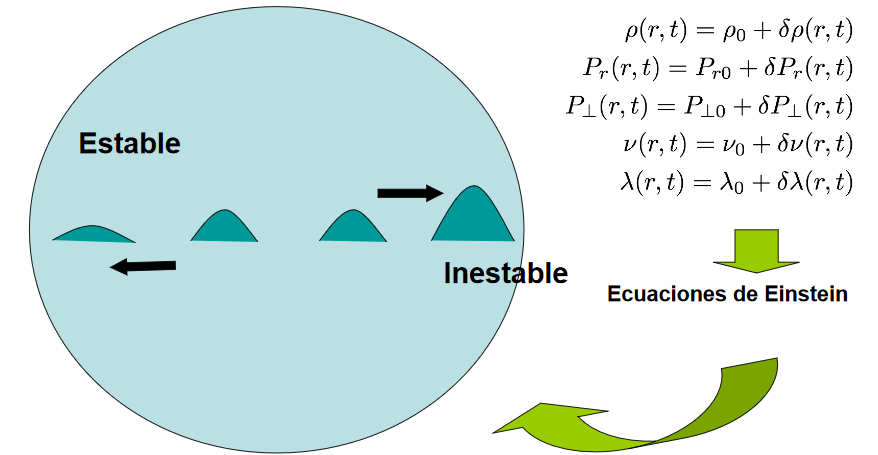
\includegraphics[width=0.8\textwidth]{Chandra.png}
\end{figure}




\vspace{3mm}


\end{itemize}




\end{frame}




\begin{frame}{Introducción e Historia - Fracturas}

\begin{itemize}

\vspace{-3mm}

\item L. Herrera (1992, 1994, 1997): Perturbación simultánea de la densidad y la anisotropía.

\vspace{1mm}

\begin{itemize}
\item Abreu - Hernández - Núñez (2007): Perturbación de la densidad $\rightarrow$ perturbación de las presiones. No se perturba el gradiente de presión.

\vspace{2mm}

\item González - Navarro - Núñez (2015): Perturbación de la densidad. Sí perturba el gradiente de presión.

\vspace{2mm}



\begin{figure}[h]
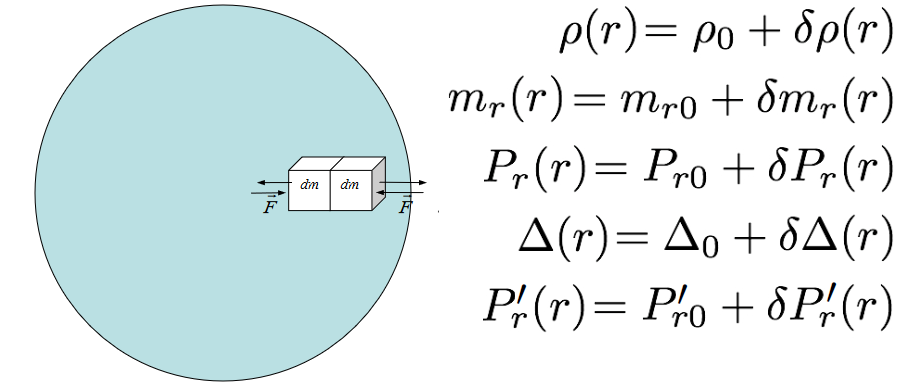
\includegraphics[width=0.8\textwidth]{Frac.png}
\end{figure}

\end{itemize}


\vspace{2mm}

 


\end{itemize}


\end{frame}





\begin{frame}{Introducción e Historia - Estabilidad Convectiva}

\begin{itemize}

\vspace{-5mm}

\item Bondi - Thorne - Kovetz (1964, 1966, 1967)
%\item Hernández - Núñez - Vásquez-Ramírez (2018)

\begin{itemize}
    \item Si $\rho_{e} > \rho_{s}$, la gravedad tenderá a atraer al elemento de fluido hacia el centro de la esfera y el sistema será inestable.
    \vspace{2mm}
    \item Si $\rho_{e} = \rho_{s}$, el sistema será metaestable.
    \vspace{2mm}
    \item Si $\rho_{e} < \rho_{s}$, el elemento de fluido retornará a su posición inicial y el sistema será estable.
\end{itemize}

\item Hernández - Núñez - Vásquez-Ramírez (2018): 
$\rho^{\prime \prime} (r) \leq 0$

\end{itemize}

\begin{figure}[h]
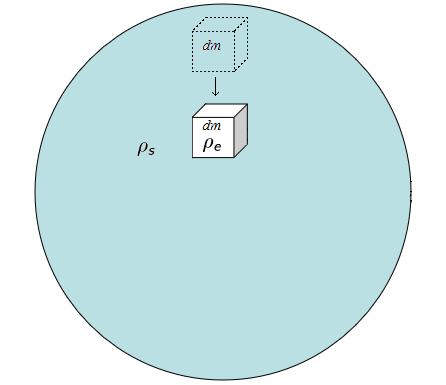
\includegraphics[width=0.5\textwidth]{Flota.png}
\end{figure}



\end{frame}




\section{Planteamiento}
\begin{frame}{Planteamiento del problema}

\vspace{-4mm}

\justifying Hernández, Núñez y Vásques-Ramírez además estudian la estabilidad bajo el concepto de fracturas para distintos modelos analíticos.

\vspace{2mm}


Encuentran que si se tiene en cuenta la reacción del gradiente de presión las inestabilidades pueden desaparecer.

\vspace{7mm}

Abreu - Hernández - Núñez \hspace{20mm} González - Navarro - Núñez

\vspace{2mm}

\hspace{18mm}$\Downarrow$ \hspace{64mm}$\Downarrow$

\vspace{2mm}

Puede presentarse fractura \hspace{22mm} No se presenta fractura

\vspace{7mm}

Sin embargo, los resultados obtenidos por González son totalmente opuestos a los propuestos por Hernández.


\end{frame}




\begin{frame}{Planteamiento del problema}

\vspace{-4mm}

\centering Hernández - Núñez - Vásquez-Ramírez: Modelo Tolman VII

\begin{figure}[h]
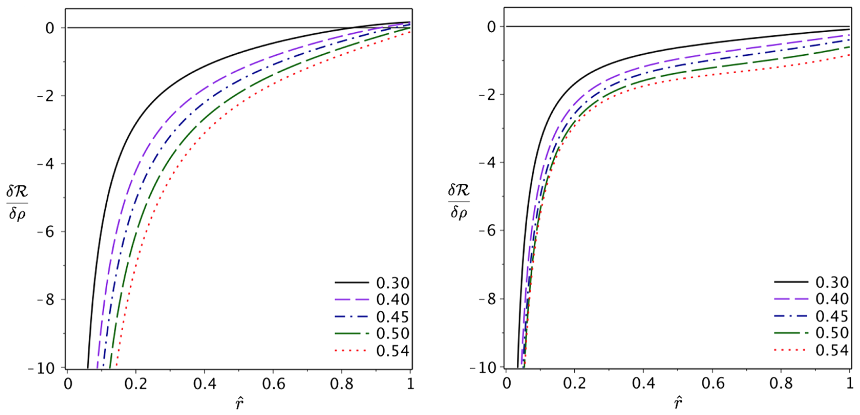
\includegraphics[width=0.85\textwidth]{FracturasConv1.png}
\end{figure}

\vspace{-8mm}

\begin{figure}[h]
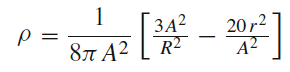
\includegraphics[width=.36\textwidth]{TolmanVII.png}
\end{figure}

\tiny H. Hernández, L. Núñez, A. Vásquez-Ramírez, The European Physical Journal C, 2018

\end{frame}



\begin{frame}{Planteamiento del problema}

\centering Hernández - Núñez - Vásquez-Ramírez: Modelo de Mehra


\begin{figure}[h]
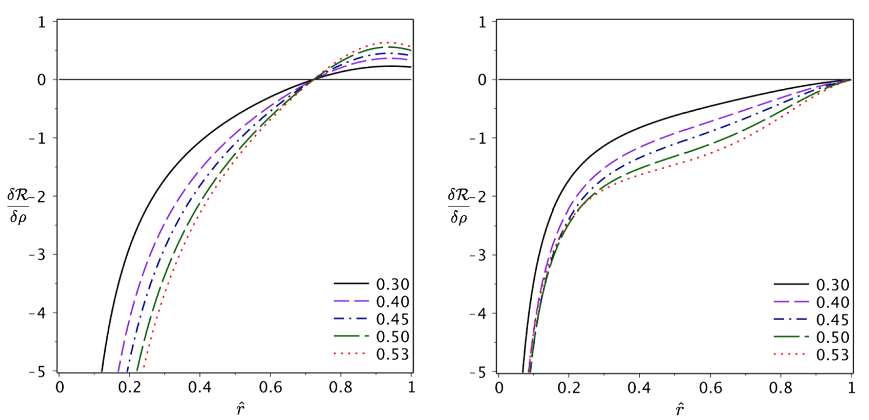
\includegraphics[width=0.8\textwidth]{FracturasConv2.png}
\end{figure}

\vspace{-3mm}

\begin{figure}[h]
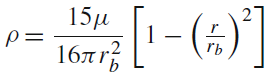
\includegraphics[width=0.36\textwidth]{Mehra.png}
\end{figure}

\tiny H. Hernández, L. Núñez, A. Vásquez-Ramírez, The European Physical Journal C, 2018


\end{frame}


\begin{frame}{Planteamiento del problema}
\vspace{-2mm}
\centering González - Navarro - Núñez : Modelo de Mehra


\begin{figure}[h]
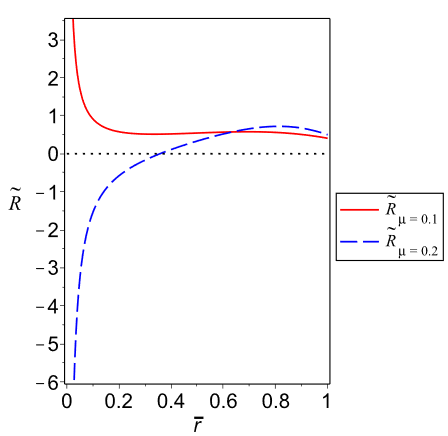
\includegraphics[width=0.55\textwidth]{Mehra2.png}
\end{figure}

\tiny G. González, A. Navarro, L. Núñez, Journal of Physics: Conference Series, 2015

\end{frame}




\begin{frame}{Planteamiento del problema}

\centering González - Navarro - Núñez:  Polítropa isótropa, $n = 2$

\vspace{-2mm}

\begin{figure}[h]
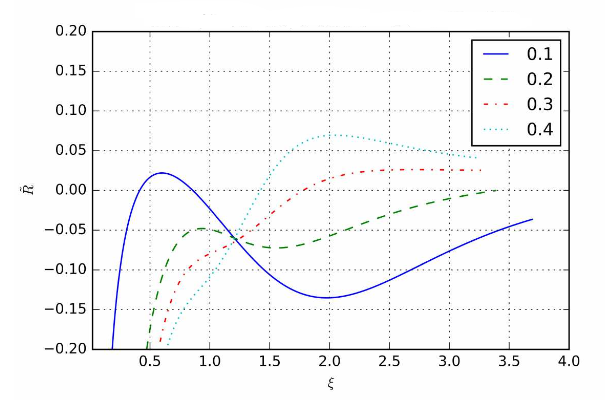
\includegraphics[width=0.75\textwidth]{FracPoliIso.png}
\end{figure}

\vspace{-2mm}

\tiny G. González, A. Navarro, L. Núñez, Journal of Physics: Conference Series, 2015


\end{frame}



\begin{frame}{Planteamiento del problema}

\centering Sharif - Sadiq : Polítropa anisótropa, $n = 2$


\begin{figure}[h]
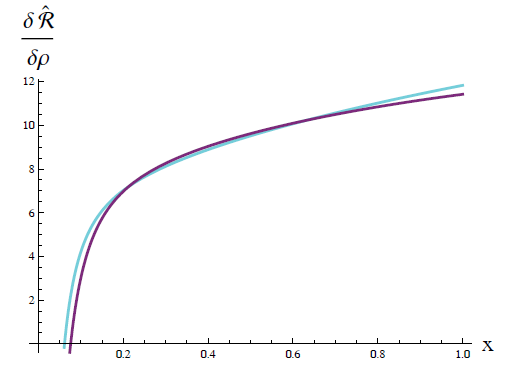
\includegraphics[width=0.6\textwidth]{Sharif.png}
\end{figure}

\tiny M. Sharif, S. Sadiq, Modern Physics Letters A, 2018


\end{frame}


\begin{frame}{Planteamiento del problema}

\justifying

Por su misma naturaleza, es posible que el concepto de fracturas y las inestabilidades convectivas tengan alguna relación.

\vspace{3mm}

Estos son criterios de estabilidad que se basan en el momento inmediatamente después de que la configuración material es perturbada.

\vspace{3mm}

Adicionalmente, se puede observar en el esquema de perturbación de fracturas que el gradiente de presión relaciona las inestabilidades convectivas con las fracturas:

\vspace{-6mm}

\begin{equation*}
\hspace{-8mm}
\scriptsize
\label{EqHidPer}
\delta \mathcal{R} = \delta \rho \left\lbrace \frac{\partial \mathcal{R}}{\partial \rho} + \frac{\partial \mathcal{R}}{\partial P} v^{2} + \frac{\partial \mathcal{R}}{\partial P_{\perp}} v^{2}_{\perp} + \frac{\partial \mathcal{R}}{\partial m} \left[ \frac{4 \pi r^{2} \rho}{\rho^{\prime}} \right] + \frac{\partial \mathcal{R}}{\partial P^{\prime}} \left[ { \left( v^{2} \right) }^{\prime} + v^{2} \frac{\rho^{\prime \prime}}{\rho^{\prime}} \right] \right\rbrace
\end{equation*}
    
\end{frame}

\section{Marco teórico}

%\begin{frame}{Condiciones de aceptabilidad física}

%\begin{itemize}

%\item Condición de energía débil (WEC): densidad de energía siempre positiva.

%\vspace{4mm}

%\item Condición de energía fuerte (SEC): la gravedad siempre es atractiva.

%\vspace{4mm}

%\item Condición de energía dominante (DEC): velocidad del flujo de energía menor que la velocidad de la luz.

%\vspace{4mm}

%\item Condición de energía nula (NEC).


%\end{itemize}
    
%\end{frame}



%\begin{frame}{Condiciones de aceptabilidad física}


%\begin{figure}[t]
%\hspace{-36mm}
%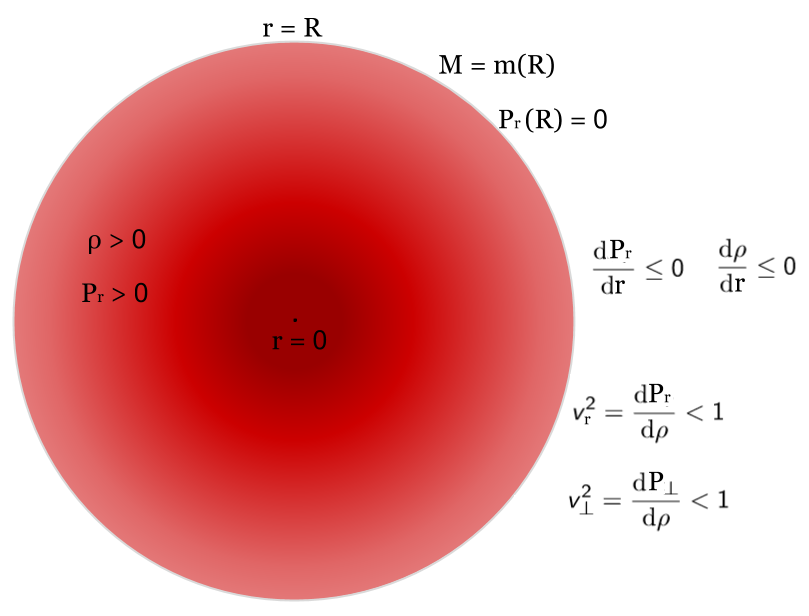
\includegraphics[width=0.8\textwidth]{Condiciones.png}
%\end{figure}
    
%\end{frame}


\begin{frame}{Ecuación de estado polítropa}

\justifying

En el caso newtoniano, la ecuación de estado polítropa está dada por:    

\begin{equation*}
\label{Poli1}
    P = K \rho_{0}^{\gamma} = K \rho_{0}^{1+1/n} \, 
\end{equation*}    

\vspace{4mm}

En el contexto de la Relatividad General se tienen dos posibilidades:

\vspace{4mm}

\begin{itemize}
    \item Caso 1: Relación entre la presión y la densidad de masa.
    \begin{equation*}
        P = K \rho_{0}^{1+1/n} \quad   \longrightarrow \quad   \rho = \rho_{0} + n P
    \end{equation*}
\end{itemize}

\tiny \centering L. Herrera, W. Barreto, Physical Review D, 2013.

\end{frame}

\justifying

\begin{frame}{Ecuación de estado polítropa}
    \begin{itemize}   
    \item Caso 2: Relación entre la presión y la densidad de energía.
    \begin{equation*}
    \label{Poli2}
        P = K \rho^{1+1/n}  \quad  \longrightarrow  \quad  \rho = \frac{\rho_{0}}{\left(1 - K \rho_{0}^{1/n} \right)^{n}}
    \end{equation*}
    
    

\end{itemize}

\vspace{4mm}

Ambos casos son una descripción relativista que representa físicamente el caso newtoniano de una polítropa, cuando $P_{c} / \rho_{c} \rightarrow 0$.

\vspace{24mm}

\tiny \centering L. Herrera, W. Barreto, Physical Review D, 2013.
    
    
\end{frame}






\begin{frame}{Condiciones de aceptabilidad física}

\justifying

C1: Potenciales métricos positivos, finitos y libre de singularidades en el interior de la esfera.

\vspace{2mm}

C2: Condiciones de acoplamiento. En la superficie de la esfera, $r=r_{b}$, la solución interior debe coincidir de forma continua con la solución exterior de Schwarzschild.

\vspace{2mm}

C3: Disminución del corrimiento al rojo interior ($Z$) al aumentar $r$.

\vspace{2mm}

C4: La densidad y las presiones no deben ser negativas dentro de la esfera.

\vspace{2mm}

C5: El máximo de la densidad y las presiones se encuentra en el centro.

\vspace{4mm}
\centering
\tiny B. Ivanov, The European Physical Journal C, 2017.


\end{frame}



\begin{frame}{Condiciones de aceptabilidad física}

\justifying

C6: Condiciones de energía. Fuerte $\rho \geq P + 2 P_{\perp}$; o Dominante $\rho \geq P$ y $\rho \geq P_{\perp}$.

\vspace{2mm}

C7: Condiciones de causalidad. La velocidad tangencial y radial del sonido no debe sobrepasar la velocidad de la luz.

\vspace{2mm}

C8: Criterio de estabilidad para el índice adiabático  $\gamma = \frac{\rho + P}{P} v^{2} \geq \frac{4}{3}$.

\vspace{2mm}

C9: Estabilidad contra fracturas. Las regiones potencialmente inestables son aquellas donde la velocidad del sonido tangencial al cuadrado es mayor que la velocidad del sonido radial al cuadrado.

\vspace{2mm}

C10: Condición de estabilidad Harrison-Zeldovich-Novikov, la cual implica que  $\mathrm{d}M(\rho_{c}) / \mathrm{d}\rho_{c} < 0 $.

\vspace{8mm}
\centering
\tiny B. Ivanov, The European Physical Journal C, 2017.

\end{frame}



\begin{frame}{Fracturas}


\begin{equation}
\label{EqHid}
 \mathcal{R} = P^{\prime}+(\rho +P)\frac{m + 4 \pi r^{3}P}{r(r-{2}m)}-\frac{2(P_\perp -P)}{r} = 0
\end{equation}

\vspace{3mm}

\begin{itemize}
\item Perturbaciones locales en la densidad
\end{itemize}

Una perturbación en la densidad, $ \rho \, \mathrm{\rightarrow} \, \rho \, {+} \,  \mathrm{\delta} \rho (r) $ , induce una perturbación de su gradiente,
\begin{equation*}
\rho^{\prime} (\rho + \mathrm{\delta} \rho) \approx \rho^{\prime} (\rho) + \delta \rho^{\prime} = \rho^{\prime} (\rho) + \frac{\mathrm{d} \rho^{\prime}}{\mathrm{d} \rho} \mathrm{\delta} \rho
\end{equation*}

\vspace{8mm}

\tiny \centering G. González, A. Navarro, L. Núñez, Journal of Physics: Conference Series, 2015

\end{frame}


\begin{frame}{Fracturas}

\vspace{-9mm}

\begin{equation}
\footnotesize
P^{\prime} (\rho + \delta \rho) \approx P^{\prime} (\rho) + \delta P^{\prime} \approx P^{\prime} (\rho) + \frac{\mathrm{d} P^{\prime}}{\mathrm{d} \rho} \delta \rho \approx P^{\prime} (\rho) + \left[ { \left( v^{2} \right) }^{\prime} + v^{2} \frac{\rho^{\prime \prime}}{\rho^{\prime}} \right]
\end{equation}

\begin{equation*}
\mathcal{R} \approx \mathcal{R}_{0} \left( \rho, P, P_{\perp}, P^{\prime}, m \right) + \delta \mathcal{R}
\end{equation*}

\begin{equation}
\label{EqHidPer}
\scriptsize
\delta \mathcal{R} = \delta \rho \left\lbrace \frac{\partial \mathcal{R}}{\partial \rho} + \frac{\partial \mathcal{R}}{\partial P_{r}} \frac{\mathrm{d} P_{r}}{\mathrm{d} \rho} + \frac{\partial \mathcal{R}}{\partial P_{\perp}} \frac{\mathrm{d} P_{\perp}}{\mathrm{d} \rho} + \frac{\partial \mathcal{R}}{\partial m} \frac{\mathrm{d} m}{\mathrm{d} \rho} + \frac{\partial \mathcal{R}}{\partial P_{r}^{\prime}} \frac{\mathrm{d} P_{r}^{\prime}}{\mathrm{d} \rho} \right\rbrace  
\end{equation}

\begin{equation}
\hspace{-8mm}
\scriptsize
\label{EqHidPer}
\delta \mathcal{R} = \delta \rho \left\lbrace \frac{\partial \mathcal{R}}{\partial \rho} + \frac{\partial \mathcal{R}}{\partial P} v^{2} + \frac{\partial \mathcal{R}}{\partial P_{\perp}} v^{2}_{\perp} + \frac{\partial \mathcal{R}}{\partial m} \left[ \frac{4 \pi r^{2} \rho}{\rho^{\prime}} \right] + \frac{\partial \mathcal{R}}{\partial P^{\prime}} \left[ { \left( v^{2} \right) }^{\prime} + v^{2} \frac{\rho^{\prime \prime}}{\rho^{\prime}} \right] \right\rbrace
\end{equation}

\vspace{10mm}

\tiny \centering G. González, A. Navarro, L. Núñez, Journal of Physics: Conference Series, 2015

\end{frame}


\begin{frame}{Estabilidad convectiva}
\justifying

\vspace{2mm}
Considerando un cubo infinitesimal con densidad $\rho (r_{p})$ que es desplazado hacia el centro de la esfera y cuya posición inicial es denotada como $r_{p}$ se tiene:

\vspace{-2mm}

\begin{equation*}
    \rho (r_{p}) \rightarrow \rho (r_{p}) + \delta \rho(r) \, , \quad \text{siendo} \hspace{3mm} \delta \rho (r) = \rho^{\prime} (r)(- \delta r) \quad \text{y} \quad r = r_{p} - \delta r \, , 
\end{equation*}

\vspace{4mm}

donde $r$ es la posición desplazada del cubo y $- \delta r$ el desplazamiento hacia el centro.

\vspace{2mm}

Por lo tanto, la densidad del cubo luego de ser desplazado siempre será mayor que al inicio.

\vspace{10mm}

\tiny H. Hernández, L. Núñez, A. Vásquez-Ramírez, The European Physical Journal C, 2018
    
\end{frame}


\begin{frame}{Estabilidad convectiva}

\justifying

Expandiendo la densidad del medio que rodea al cubo desplazado se tiene:
    \begin{equation*}
    \rho (r_{p} - \delta r) \approx \rho (r_{p}) + \rho^{\prime} (r_{p})(- \delta r) \, 
\end{equation*}

El sistema será estable bajo convección si la densidad del medio es mayor o igual que la densidad del cubo, entonces:

\vspace{-4mm}

\begin{equation*}
\hspace{-6mm}
    \rho(r_{p}) + \rho^{\prime} (r_{p})(- \delta r) \, \geq \, \rho(r_{p}) + \rho^{\prime}(r)(- \delta r) \, \, , \quad \text{y por lo tanto} \hspace{3mm} \rho^{\prime}(r_{p}) \leq \rho^{\prime}(r)
\end{equation*}

Finalmente, expandiendo $\rho^{\prime}(r)$ alrededor de $r_{p}$ se tiene:

\begin{equation*}
    \rho^{\prime}(r_{p}) + \rho^{\prime \prime} (r_{p}) \delta r \, \leq \, \rho^{\prime}(r_{p}) \quad \Rightarrow \quad \rho^{\prime \prime} (r) \leq 0 \, 
\end{equation*}

\vspace{6mm}

\tiny H. Hernández, L. Núñez, A. Vásquez-Ramírez, The European Physical Journal C, 2018

\end{frame}






\section{Objetivos}
\begin{frame}{Objetivos}
\vspace{10mm}
Objetivo general: \\
\vspace{8mm}
\justifying
Comparar y explorar la posibilidad de establecer una relación entre la estabilidad convectiva y el concepto de fracturas en esferas autogravitantes polítropas anisótropas en el marco de la Relatividad General. \\

\end{frame}


\begin{frame}{Objetivos}


Objetivos específicos:
\vspace{4mm}
\begin{itemize}
\justifying
\item Caracterizar modelos polítropos y estudiar su estabilidad bajo inestabilidades convectivas y bajo el concepto de fracturas.
\vspace{2mm}

\item Identificar cuáles valores del índice polítropo $n$, para las ecuaciones de estado polítropas, cumplen con condiciones de aceptabilidad física.
\vspace{2mm}

\item Comparar los criterios de estabilidad desarrollados.
\vspace{2mm}

\item Establecer si existe relación entre estabilidad convectiva y fracturas.

\end{itemize}



\end{frame}






\section{Hipótesis}
\begin{frame}{Hipótesis}

\vspace{14mm}

\justifying
La reacción del gradiente de presión ante perturbaciones locales de la densidad impide la aparición de fuerzas que cambien de signo dentro de la configuración
material, justo después de que esta abandone el equilibrio hidrostático.



\end{frame}

\section{Metodología}
\begin{frame}{Metodología}
\justifying

1. Modelado de la configuración material a través de las ecuaciones de estructura y conservación de la masa. \\
\vspace{4mm}
\pause
2. Integración numérica del sistema de ecuaciones para distintos valores del índice polítropo $n$. \\
\vspace{4mm}
\pause
3. Análisis de estabilidad bajo el concepto de fracturas y cálculo de la segunda derivada de la densidad. \\
\vspace{4mm}
\pause
4. Análisis de estabilidad convectiva. \\
\vspace{4mm}
\pause
5. Comparación entre los dos criterios de estabilidad desarrollados para establecer una relación entre ellos.
\end{frame}


\section{Cronograma}
\begin{frame}{Cronograma}

\begin{figure}
\centering
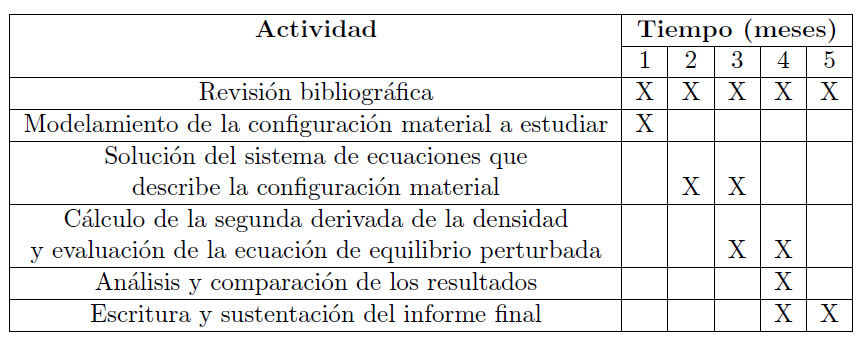
\includegraphics[width=1\textwidth]{Cronograma.png}
\end{figure}

\end{frame}





\begin{frame}
\vspace{36mm}
\hspace{42mm}
				PREGUNTAS
\end{frame}


\begin{frame}
\vspace{36mm}
\hspace{47mm}
				¡GRACIAS!
\end{frame}


\end{document}